\documentclass{article}

\usepackage{neurips_2020_author_response}

\usepackage[utf8]{inputenc} % allow utf-8 input
\usepackage[T1]{fontenc}    % use 8-bit T1 fonts
\usepackage{hyperref}       % hyperlinks
\usepackage{url}            % simple URL typesetting
\usepackage{booktabs}       % professional-quality tables
\usepackage{amsfonts}       % blackboard math symbols
\usepackage{nicefrac}       % compact symbols for 1/2, etc.
\usepackage{microtype}      % microtypography
\usepackage{subcaption}
\usepackage{graphicx}
\usepackage{wrapfig}

\begin{document}

First, thank all the reviewers for offering valuable suggestions to help to improve the writing of the paper.
The reviewers generally agree that our paper is innovative in some aspects, but needs some improvement in the writing.

Reviewer \#1 think our work lack the comparison to strong baselines like TensorFlow and PyTorch.
This is not true, Tapenade is a very strong baseline in the field of \textbf{generic} AD.
TensorFlow and PyTorch are \textbf{domain specific} AD software for traditional tensor-based machine learning.
Some applications like the bundle adjustment in computer vision mainly contains scalar operations.
People benchmarked the speed of obtaining Jacobians with different packages as shown in the figure, which suggests that we have chosen one of the worlds' best generic AD package as our baseline.
\begin{wrapfigure}{l}{0.5\textwidth}
    \centerline{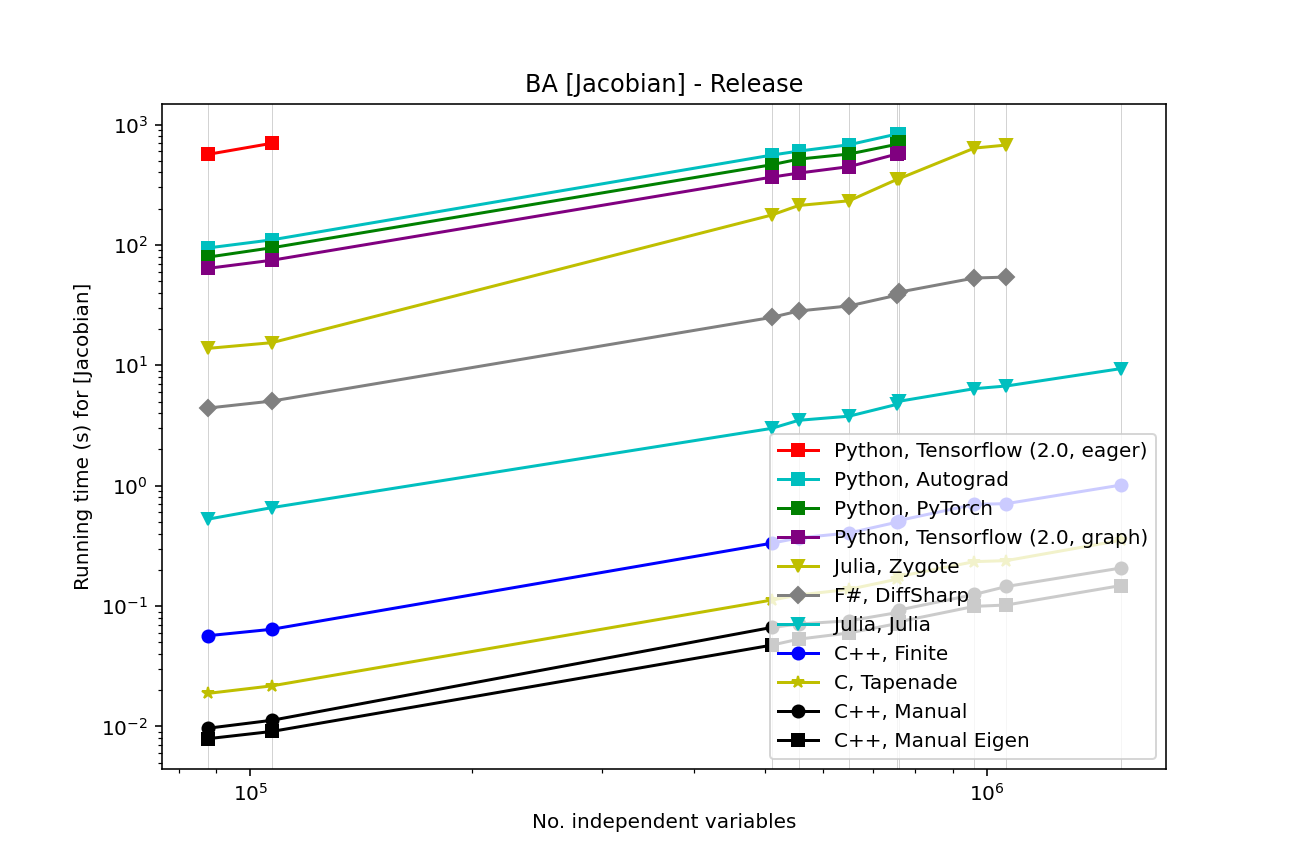
\includegraphics[width=0.5\columnwidth,trim={0 1cm 1cm 1.7cm},clip]{ba-jacobian-adbench.png}}
    \caption{The bundle adjustment benchmark conducted by the ADBench (from the github) project of microsoft [arXiv:1807.10129]. NiLang outperforms all software in this figure.}\label{bench-ba}
\end{wrapfigure}
Tapenade is $10^{3-5}$ times faster than PyTorch and TensorFlow. However Tapenade is commercial, close sourced and C/Fortran based.
We are proud that NiLang is even better than Tapenade in this benchmark.
We don't benchmark the popular Julia package Flux because we benchmarked its backend Zygote instead, where NiLang shows more than one order advantage in time.

Reviewer \#2 is wondering if reversible computing is equivalent to traditional AD with optimized checkpointing.
We agree that with \textit{proper coding style} and the use of reversibility, optimal checkpointing is equivalent to reversible programming.
However, the \textit{proper coding style} is very difficult for a user without reversible thinking in mind.
In the sparse matrix dot product example in the Appendix.
NiLang requires a user to preallocate a \texttt{branch\_keeper} to store the decisions of branches to enforce reversibility inside the loop.
However, if a user is writing it in free style, checkpointing has to insert stack operations inside the loop, which will slow down the program significantly.
Not to say the optimal checkpointing itself is a well known hard topic.
Allocating automatically for a user is even more dangerous in GPU programming.
In NiLang, one can compile the bundle adjustment code to GPU to enjoy a ~200x speed up with no more than 10 extra lines of code.
It is much easier for users to completely avoid allocation inside a loop in NiLang comparing with checkpointing.
Allocation can be the performance killer when differentiating array mutation operations.
NiLang supports array mutations naturally. As NiLang is getting more users, some use it to differentiate backtest policies and variational mean field computing. In both cases, NiLang help increases the performance by a factor of $\sim600$ comparing with Zygote, just because the array mutations is properly handled.
As far as we know, computational graph is not convenient to represent inplace operations.
Either the write-once \texttt{TensorArray} in TensorFlow or the mutable leaf tensors in PyTorch are not truly mutable.
This explains Referee \#4's concern that the computational graph can represent any program.
Yes, but they are not convenient to describe array mutations.

%One of the reviewer mention that to handle the backward rule of ``+'' operation, one do not need to store the inputs of an instruction, gradient of both inputs are $1$. There is no need to trace back the state. We haven't put effort in optimizing such operations yet.
%In NiLang, the backward propagation program generally contains $\sim2$ times more instructions than the forward pass. This factor is estimated by considering the backward rule of the multiplication operation. This is a known bottleneck in the field of generic AD.

Reviewer \#3 wants to know from which aspect NiLang is different from a traditional reversible programming language, and the limitations of the reversible programming AD.
For a long time, the reversible programming languages focus mainly on the theoretical elegance and ignored the productivity. Researchers tried to add functional and object-oriented features to reversible languages.
NiLang is special for that it supports many practical elements like arrays, complex numbers, fixed-point numbers, and logarithmic numbers and being an eDSL so that it can be used directly to accelerate machine learning frameworks in Julia.
Reversible programming does not have any limitation in describing a computational process, because any program can be written in a reversible form. The most severe weakness of NiLang should be the floating-point arithmetic suffers from the rounding error.
We add a seperate section to help people understand the limitations and possible solutions better.

Reviewers \#1 and \#4 think our result can not be reproduced. Considering both NiLang and the benchmarks are open source on GitHub, we respectfully disagree.
Reviewer \#1 mention that SVD is available in PyTorch and TensorFlow. It is true. There are more than 10 papers on differentiating SVD and we cited some of them in the main text. We emphasis that SVD backward rules are \textbf{manually} generated. We say, ``Why bother 10 papers? Just let the generic AD do its job!''
%comparing reversible programming and the reversible neural networks in the main text directly. Thanks for your valuable information.

At last, we encourage reviewers to view this project more from the ``future'' perspective.
Nowadays, energy is becoming one of the most deadly bottlenecks for machine learning applications.
From a physicist's perspective, we believe that reversible computing is the only correct approach to solve energy conundrums.
Classical reversible computing has been silenced for $\sim$15 years, NiLang is trying to bridge the new trend machine learning and reversible computing.
We will try our best to convey this point better in the updated manuscript. As Reviewer \#2 said, it is a long overdue.


\end{document}
